\documentclass[logo,dosguias,magister,propuesta]{tesis-postgrado}
% opciones: logo,dosguias,magister,doctorado,propuesta,txfonts

\keywords{XML; Key Implication}

\begin{document}
\baselineskip 23pt
% ----------------------------------------------------------
% ----------- PARTE INICIAL --------------------------------
\thispagestyle{empty}
% Rellenar con la informacion personal y del trabajo

\titulo{Claves XML: Una Implementaci\'on de Algoritmos de Implicaci\'on y Validaci\'on}

\autor{Emir Fernando Mu\~noz Jim\'enez}
\email{emir.munozj@usach.cl}
\telefono{8752 9608}
\run{16.269.030\-2}
\annoingreso{2009}

\fecha{Lunes}{30}{Mayo}{2011}

\director{Dr.\ Mauricio Mar\'in}
\codirector{Dr.\ Flavio Ferrarotti}

\ciudad{Santiago}
\pais{Chile}

\makecubierta


\makecopyright % si es propuesta no se mostrará
% ----------------------------------------------------------
% ----------- PRIMERA PARTE --------------------------------
\frontmatter
% ### Resumen e Indices ####

\begin{gracias}

\end{gracias}

\dedicatoria{
  A mi\ldots
}


\resumenCastellano{
La flexibilidad sintáctica, y el complejo anidamiento de los datos en una estructura tipo árbol 
dificulta expresar propiedades deseables de los datos XML, ofreciendo una capacidad limitada para 
expresar semántica. En esta tesis se presenta un estudio de las claves como restricciones de 
integridad sobre documentos XML, implementando algoritmos para los problemas de implicación y 
validación, con el fin de mostrar la factibilidad de usar las capacidades semánticas que éstas 
entregan, y que XML como modelo requiere.
\vspace*{0.5cm}
\KeywordsES{XML; Claves XML; Implicación de claves; Validación de documentos XML; Cover no redundante}
}

\newpage

\resumenIngles{
The syntactic flexibility and complex tree-like nested data make it challenging to express desirable 
properties of XML data, offering a limited capability to express semantic. In this thesis, we present 
a study of keys as integrity constraints on XML documents, implementing algorithms for implication 
and validation problems, with the aim of showing the factibility of using the semantic capabilities 
that keys gives and XML as a model requires.
\vspace*{0.5cm}
\KeywordsEN{XML; XML keys; Key implication; XML document validation; Non-redundant cover}
}

\pagestyle{fancy}
\fancyhead[L]{\slshape \leftmark}
\fancyhead[C]{}
\fancyhead[R]{\thepage}
\tableofcontents        %% Indice general
\listoffigures          %% Indice de figuras
\listoftables           %% Indice de tablas
\listofalgorithms       %% Indice de algoritmos
% ----------------------------------------------------------
% ----------- SEGUNDA PARTE --------------------------------
\mainmatter
% ### Configuración del header ###
\pagestyle{fancy}
\fancyhead[L]{\slshape \leftmark}
\fancyhead[C]{}
\fancyhead[R]{\thepage}
\pagenumbering{arabic}
% ### Capitulos de la tesis ###
\chapter{Introducci\'on}
\label{cap:intro}

\section{Antecedentes y motivaci\'on}
\label{intro:motivacion}

El rápido desarrollo de la Web ha generado nuevos problemas y áreas de investigación en las Ciencias de la Computación e Informática. Junto a eso ha iniciado el desarrollo de (innumerables) nuevas tecnologías, y la evolución de otras. La comunicación e interoperabilidad de estas tecnologías es un tema crucial para mantener el desarrollo de la Web. En particular, XML (\textit{eXtensible Markup Language} o Lenguaje extensible de marcado) ha surgido como un modelo de datos estándar para almacenar e intercambiar datos en la Web. Su rol en el intercambio de datos ha pasado de simplemente transmitir la estructura de los datos, a uno que también transmite su semántica \citep{Benedikt:2003, Davidson:2007}.

XML \citep{XML:2006} es la propuesta del \textit{World Wide Web Consortium} (W3C) como lenguaje de intercambio e interoperabilidad en la Web. Este lenguaje proporciona un alto grado de flexibilidad sintáctica, pero ofrece una capacidad limitada para expresar la semántica de los datos. Esta flexibilidad sintáctica, y el complejo anidamiento de los datos en una estructura tipo árbol, dificulta expresar propiedades deseables de los datos XML. En consecuencia, el estudio de restricciones de integridad ha sido reconocido como una de las áreas de investigación en XML más difíciles \citep{Fan:2005,Suciu:2001,Vianu:2003,Widom:1999}.

El estudio de restricciones de integridad ha sido reconocido como una de las áreas más difíciles de investigación en XML \citep{Vianu:2003}. En el modelo relacional, las restricciones han sido estudiadas extensamente \citep{Fagin:1984, Thalheim:1991}, y son esenciales para el diseño de esquemas, la optimización de consultas, y métodos eficientes de acceso y almacenamiento \citep{Abiteboul:1995}. Varias clases de restricciones de integridad han sido definidas para XML, incluyendo claves \citep{Buneman:2002}, restricciones de camino \citep{Buneman:2001,Buneman:2000}, restricciones de inclusión \citep{Fan:2002,Fan:2003}, y dependencias funcionales \citep{Arenas:2004,Hartmann:2006,Vincent:2004}. Sin embargo, la mayoría de las clases de restricción, dada la compleja estructura de datos XML, resultan en problemas de decisión que son intratables, y es difícil encontrar clases de restricciones XML que sean naturales y útiles, y que puedan ser razonadas de manera eficiente \citep{Fan:2005,Fan:2003,Fan:2002,Suciu:2001,
Vianu:2003,Arenas:2002}. Las principales candidatas de esas clases son las claves absolutas y relativas \citep{Buneman:2003,Buneman:2002} que son definidas en base a un modelo de árbol para XML como el propuesto por DOM \citep{DOM:1998} y XPath \citep{XPath:1999}, de manera independiente a alguna especificación del tipo\footnote{Un \textit{tipo} en XML es considerado como una gramática extendida libre de contexto, asociada a restricciones en la estructura de los elementos de un documento.} de un documento XML como DTD\footnote{\textit{Document Type Definition} o Definición de tipo de un documento XML.} o XML \textit{Schema} \citep{XMLSchema:2004}. \ldots 


\section{Descripci\'on del problema}
\label{intro:problema}

La definición de claves XML es más compleja que en el modelo relacional, debido a la compleja estructura de árbol que poseen los documentos XML.

En este trabajo se plantea, en primer lugar, determinar la utilidad de trabajar en la práctica con claves XML utilizando un algoritmo para el problema de implicación. Definir ésta utilidad práctica permitirá avanzar en la aceptación de las claves como restricciones sobre XML por parte de los profesionales, considerando el poder expresivo que estas entregan a XML. En segundo lugar, existe la necesidad de un método que permita  determinar la validez de un documento XML contra un conjunto predefinido de claves XML. A partir de los trabajos realizados en validación de documentos XML contra claves \citep{Abrao:2004, Bouchou:2003, Chen:2002, Liu:2005, Liu:2004}, se plantea diseñar un algoritmo que permita validar documentos XML contra claves XML como las definidas en \citet{Buneman:2003,Buneman:2002}, las cuales consideran la igualdad en valor entre nodos elemento: si los subárboles que tienen por raíz a estos nodos, son isomorfos por algún isomorfismo que para cadenas de texto se corresponde con la función 
identidad.

Finalmente, considerando que la complejidad del algoritmo de validación depende en parte del tamaño del conjunto de claves, se investiga un método para obtener una optimización del proceso de validación de documentos XML contra claves, utilizando el algoritmo de implicación de claves XML presentado por \citet{HartmannLink:2009}.

\section{Soluci\'on propuesta}
\label{intro:solucion}


\section{Objetivos y alcance del proyecto}
\label{intro:objetivos}

\subsection{Objetivo general}


\subsection{Objetivos espec\'ificos}

Para la consecución del objetivo general, se plantean las siguientes metas intermedias:

\begin{enumerate}
  \item Estudiar la noción de claves XML y las axiomatizaciones existentes.
  \item 
\end{enumerate}

\subsection{Alcances}


\section{Metodolog\'ia y herramientas utilizadas}
\label{intro:metodologia}

\subsection{Metodolog\'ia}


\subsection{Herramientas de desarrollo}


\section{Resultados Obtenidos}
\label{intro:resultados}


\section{Organizaci\'on del documento}
\label{intro:organizacion}

El presente trabajo está dividido en ocho capítulos considerando éste como el primero. En el Capítulo~\ref{cap:preliminares} se formalizan los fundamentos de documento XML, modelo de árbol XML, y lenguaje de definición de expresiones de camino para definir claves XML. \ldots

%--------Preliminares
%--------Emir Muñoz Jiménez
%--------13-10-2010

\chapter{Marco Te\'orico}
\label{cap:preliminares}


\section{Documentos XML}


% Figura: \'Arbol XML 1
\begin{figure}[tp]
  \centering
  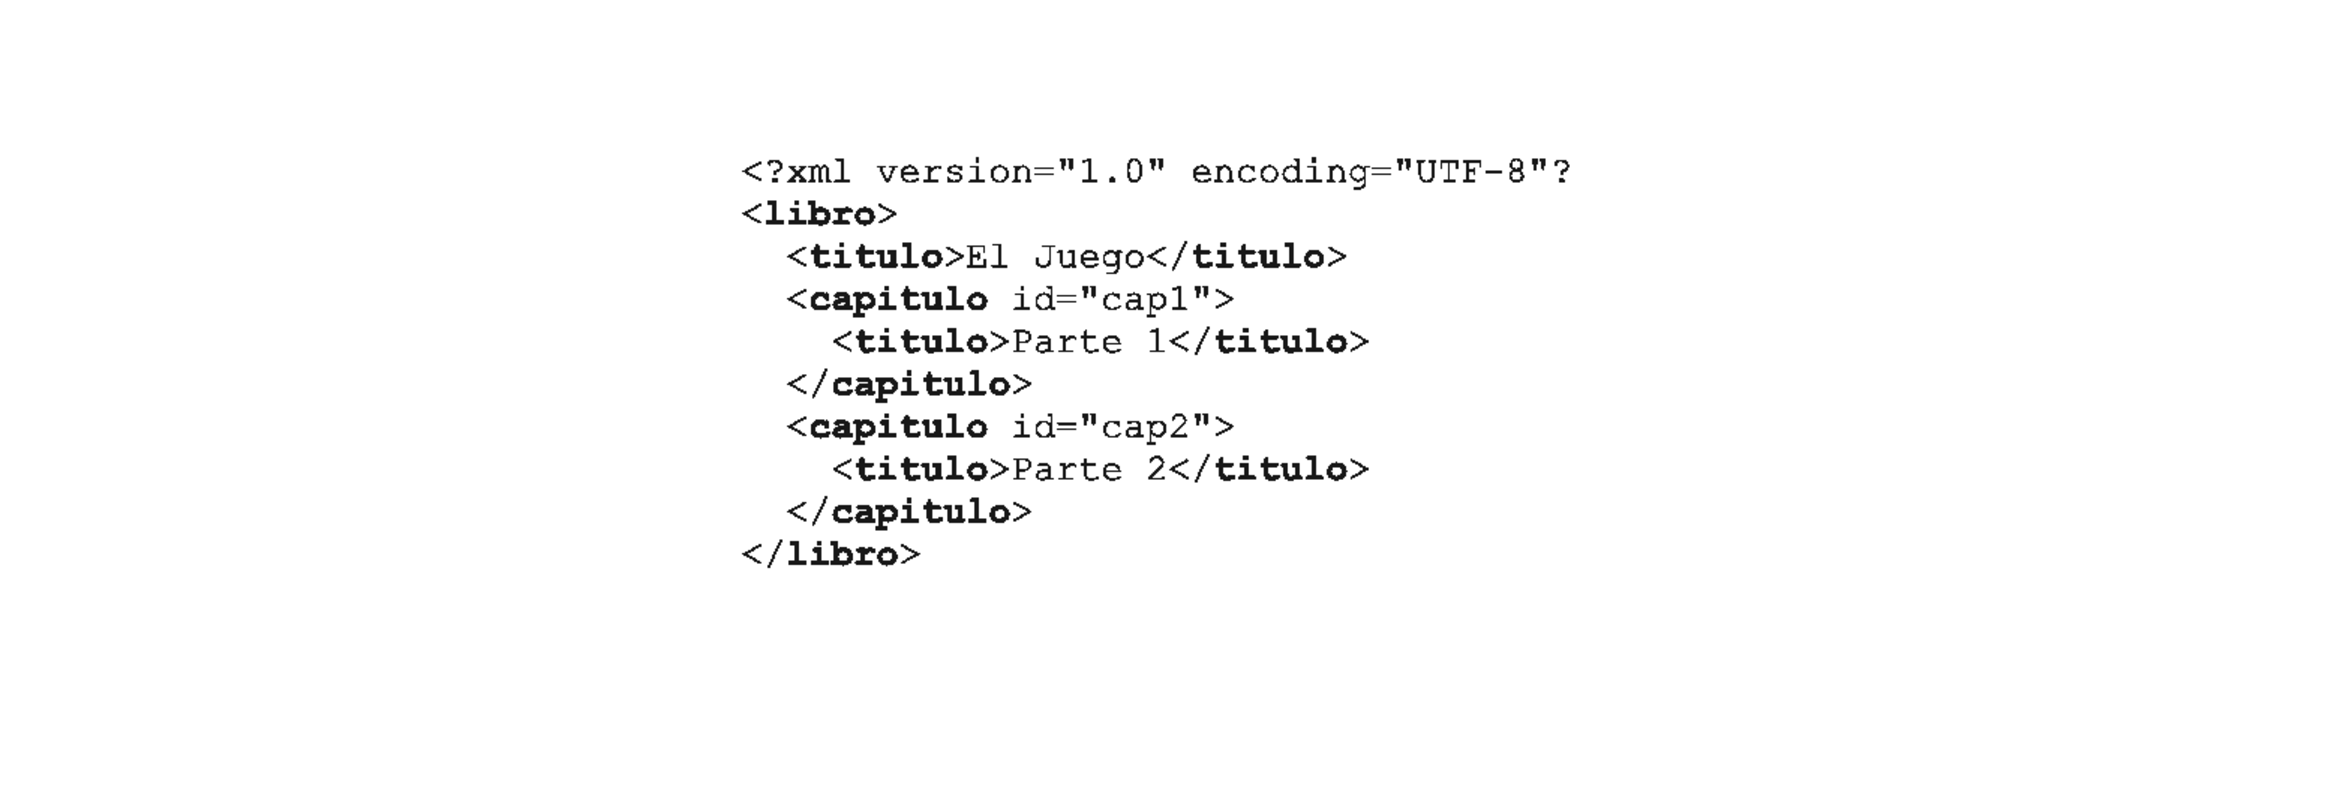
\includegraphics[scale=.5]{images/XML-document-example1}
  \caption{\em Modelo de árbol para un documento XML.}
  \label{fig:xml-tree-exa1}
\end{figure}

\section{El modelo de \'arbol XML}

% ----------------------------------------------------------
% ----------- TERCERA PARTE --------------------------------
% \backmatter %Elimina la numeración
% ### Bibliografía de este documento ###
\bibliographystyle{apa-good}
\bibliography{referencias}
% ----------------------------------------------------------
% ----------- CUARTA PARTE ---------------------------------
\appendix
\addappheadtotoc %agregar Apéndice al índice. Si no tiene apéndices COMENTAR o BORRAR
% \noappendicestocpagenum %quitar número de páginas a los apéndices
% ### ANEXOS ###
%--------Apendice
%--------Emir Muñoz Jiménez
%--------13-10-2010

\chapter{Manual de Usuario}
\label{cap:manual}


\section{Requerimientos}

blablablabla....

\section{Instalaci\'on}

blablablabla....

blablablabla....
 % Manuales de Usuario
\end{document}
%\\end
